
\chapter{Introduction}

With the world constantly evolving day to day, people want to understand what is happening. To properly understand something, one needs to analyze data. In today's age, the~volume of the produced data rises exponentially. The term Big Data was first coined in~2005 and was a direct consequence of the development of Web 2.0. Many distributed frameworks were developed with the need to process data that contains greater variety, arriving in increasing volumes and with more velocity. One of these frameworks is Apache Spark. The successor to Apache Hadoop's Map Reduce uses an innovative programming model for~distributed data processing. Chapter \ref{chap:spark} describes Spark in more detail and mentions some details and workflows necessary for this thesis. 

As the volume of the data increases, the need to develop applications in processing frameworks follows the same trend. To reduce the necessary work to develop these applications, people search for an optimization. One possible approach is to formalize the~design and then automate the development. A Model-Driven Development approach introduces a~way to develop software using graphical modeling. Afterward, the source code of~the~application is generated. An overview and advantages of Model-Driven Development and~Model-Drive Architecture can be found in chapter \ref{chap:mdd}.

This thesis' motivation is to design a method to formally model Big Data processing tasks in Spark and implement the solution. With the rundown of the essential concepts out of the way, the next chapter \ref{chap:existing} describes the related and already existing work in this field. Previous projects offer inspiration but also an insight into what can be improved. 

Chapter \ref{chap:design} goes over the proposed meta-model design while describing it in detail. Analyzing the previous solutions turned out the already existing ecosystem for modeling is designed with extensibility in mind. The meta-model to describe Spark tasks is an extension of the UML Class diagram using the UML Profile diagram. By using already established tools, the meta-model becomes easier to extend and also learn. 

The aim of chapter \ref{chap:impl} is to take a closer look at the implementation of the code generator in Eclipse Acceleo. Acceleo implements the "MOFM2T" standard, from the Object Management Group, for performing the model-to-text transformation. The generator consists of OCL templates and Java services and produces any text from a model input.

In the last chapter \ref{chap:testing}, I evaluate the proposed meta-model and the implementation of~the~generator using sample test cases. The first test is a Word Count application often considered to be the \textit{"Hello, World!"} program for Big Data processing. The next test case is the Page Rank algorithm used by Google Search. This case focuses on presenting more features and the possibility of modeling a more complex task. Finally, the last example showcases the use of the remaining features and type system using Spark's datasets.


\chapter{Apache Spark}
\label{chap:spark}

Apache Spark is an open-source framework that enables data scientists, data engineers, and machine learning engineers to run large-scale data processing distributed across a cluster, mainly Big Data processing. It ensures necessary features, such as data parallelism and fault tolerance. Spark provides expressive and intuitive API for several popular languages - Python, Scala, Java, SQL, and R. The Spark ecosystem also offers many tools and settings to make Big Data processing more straightforward. One of these tools is a command-line interface in Python and Scala used for quick ad-hoc data analysis and simple applications. It was designed to effectively support various types of workloads - batch processing, stream processing, interactive queries and interactive algorithms, machine learning training, and graph analysis. That means Spark is a good choice for developers since they only need to~use one engine for multiple types of data processing.

\section{Apache Hadoop Map Reduce}

Spark is considered a successor to Map Reduce of the Apache Hadoop framework. Both technologies analyze Big Data, but their approach is very different. Apache Spark claims to be 3X - 100X faster than Map Reduce  \cite{HadoopSpark}.

To understand the differences between these two popular processing engines, let us look at Map Reduce. Hadoop's Map Reduce distributed processing is as simple as three operations or steps. 

\begin{itemize}
    \item \textbf{Map}: each worker node inside a cluster applies the \texttt{map} function and produces new data stored in temporary storage.
     \item \textbf{Shuffle}: Worker nodes now redistribute data created by map in the previous step with their output key.
     \item \textbf{Reduce}: workers now apply the \texttt{reduce} function on shuffled data.
     
\end{itemize}



Because of the simple nature of this approach, multiple aspects might be improved upon. First, the Map Reduce API is too complicated and requires a lot of boilerplate code. Secondly,  it lacks the possibility of combining other data processing workloads such as machine learning tasks or stream processing. Finally, complex data processing tasks need to chain multiple Map Reduce operations. That makes Map Reduce tasks very disk dependent. The data are written back to the local disk of each worker node after every Map Reduce stage.





\section{Spark's design and architecture}

To improve these shortcomings, other data processing frameworks were developed. One of these frameworks is Spark which uses a multi-stage approach to distributed processing instead of a two-stage one. Spark uses in-memory storage after each computation. Also, it includes libraries for workloads such as interactive queries (Spark SQL), real-time data stream processing (Structured Streaming), machine learning (MLlib), and graph processing (GraphX).  Under the hood, Spark constructs a directed acyclic graph for its computation. 

Spark's design philosophy centers around four key characteristics \cite{LearningSpark}.


\subsection*{Modularity}


As mentioned above, Spark operations can be applied across many types of workloads and written in any of the supported programming languages mentioned above. In addition, Spark also provides highly documented libraries that include the following modules - Spark SQL, Spark Streaming, MLlib, and GraphX. 

These modules can all be used together in a single application without the need to learn different engines and libraries to process the desired task.


\subsection*{Extensibility}

Spark design focuses on its fast in-memory processing engine. That makes decoupling of~computation engine and storage possible. Moreover, since the storage is wholly decoupled, an extensive range of input data sources can be used - such as Apache Hadoop, Apache Cassandra, Apache HBase, MongoDB, Apache Hive, Apache Kafka, cloud storages Azure Storage and Amazon S3. 

The community even maintains a list of libraries that enriches the Spark ecosystem. That would not be possible if Spark's design was not extensible or easy to use.

\subsection*{Ease of use}

Using Spark, one can build Big Data processing applications with a simple programming model in popular languages. The primary abstraction of data is called Resilient Distributed Dataset (RDD). RDDs bring simplicity to the API. Higher data abstractions are constructed upon it - DataFrames and Datasets. Programming Spark application is then simply using actions and transformations on these data structures.

I will describe the Resilient Distributed Dataset and other data abstractions below in~more detail \ref{sec:rdd}.

\subsection*{Speed}

As already mentioned, Spark outperforms Hadoop in speed. Futhermore, Spark is able to utilize computer hardware thanks to its fundamental architecture design fully. Spark transforms computations to directed acyclic graphs (DAG). DAGs are then processed and optimized by graph algorithms and redistributed to worker nodes across the cluster for~parallel execution.

\pagebreak

\subsection{Spark architecture}

As already mentioned, Spark is a distributed data processing system. That means multiple machines inside a cluster collaborate to execute the submitted task. Let us take a look at the architecture of this distributed engine \cite{Sparkdip1} \cite{githubbook}. Spark uses a standard master/worker pattern shown in \ref{fig:architecture}. 

\begin{itemize}
\item \textit{Driver} - The machine responsible for initiating the computation. This machine has multiple roles. First, it is responsible for instantiating and hosting the \texttt{SparkContext} inside its JVM process. Second, it requests resources from~the~cluster manager node, such as memory or CPU. Finally, it transforms Spark code into DAG and distributes it to worker nodes. 
That means the driver is responsible for coordinating workers and the overall execution of submitted tasks. 

\item \textit{Cluster manager} - is the master node of a cluster. It manages the resources of workers and makes them run the executor program. Spark is compatible with multiple implementations of cluster managers closely described in \ref{sec:managers}.
\item \textit{Workers} - also known as slaves - are responsible for executing the calculation. They are the compute nodes where the executor program lives. When the \texttt{SparkContext} is initialized each worker node starts its executor (JVM process). This process does not stop after every step and waits for more commands from the driver. Thanks to~this Spark worker nodes are able to compute received operations of constructed DAG faster. 

The fact that the executor is a JVM process makes both horizontal(multiple worker nodes) and vertical (multiple executors on a single node) scalability possible.

\end{itemize}



\begin{figure}[H]
\centering
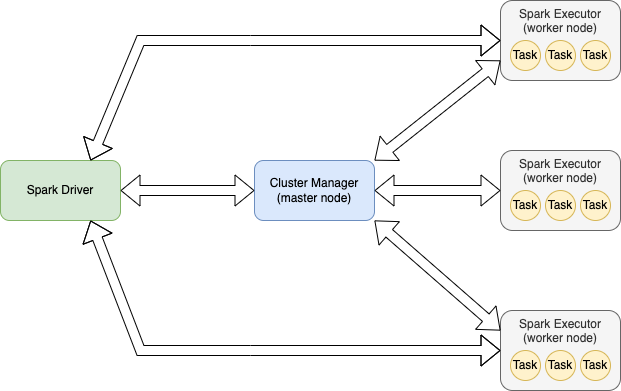
\includegraphics[width=0.8\textwidth]{obrazky-figures/spark-architecture.png}
\label{fig:architecture}
\caption{Cluster architecture of Apache Spark nodes}
\end{figure}

\pagebreak

\subsection{Spark ecosystem}

Spark creators have won a prestigious award for one of their publications, describing Spark as~a~"Unified Engine for Big Data Processing" \cite{unified}. As shown in \ref{fig:ecosystem}, Sparks unified stack offers multiple modules, cluster managers, and APIs. Unlike all the other processing frameworks, Spark unifies all components under a single engine. Although Sparks contains its own modules, it is still possible to develop open-source libraries or packages - \url{https://spark-packages.org/}. All of these modules are separate from the core computational fault-tolerant engine. That means every Spark application, whether using all or no modules or written either in Python or Scala, is still processed and decomposed into DAG, which the~Spark core executes. 
Using a modular ecosystem brings multiple advantages. The first is the nature of the layered structure. If a component on the lower level is optimized, all the~components on any higher level become faster as well.
Second, modules were designed to be highly compatible. As a result, when developers need to integrate multiple workloads, they need to set up and maintain only one system. That reduces a lot of cost and time to~use.

Now let us talk about the parts in more detail.

\subsection*{Spark Core}


Spark Core is the base of Spark functionality. It is responsible for the main features of~Spark - task dispatching, memory management, communication with the data sources, and much more. It is also the place that provides the specialized data structure called RDD (Resilient Distributed Datasets) \ref{sec:rdd}.
Spark Core offers API for this structure.

\subsection*{Spark SQL}


Spark SQL is used to work with structured data. It offers an abstraction built on RDD called DataFrame. This structure offers more information about the data than the RDD interface.
That means Spark SQL is able to optimize the calculations and store them in~permanent or temporary tables. Spark also supports SQL and HQL (Hive Query Language) used in~Apache Hive. Sparks SQL also follows standard \footnote{https://en.wikipedia.org/wiki/SQL:2003} and can be used as a pure SQL engine.
Thanks to this module, one can read data stored in various RDBMS or structured file formats such as CSV or JSON.


\subsection*{Spark Streaming}

Big Data is often created in real-time, and there is a need for real-time stream processing. Spark Streaming is a module that solves this issue. It provides an API to manipulate and process stream data similar to the Spark Core RDD fault-tolerant usage. The advantage of~this module is that developers can use both stream and static data inside a single application. For example, they can treat logs from a web server as they would static data inside a table. Also, streams can be consumed from various data sources such as Kafka, Kinesis, HDFS, or Twitter. This is a perfect example of Spark's ease of use and modularity.



\subsection*{MLlib}

With the rise of machine learning (ML) and its computational heavy training algorithms, Spark also implemented the support to distribute the computation to multiple machines. MLlib also contains a new data abstraction called Dataset. Dataset APIs offer multiple algorithms, including classification, regression, decision trees, clustering, and many more. As mentioned above, Spark is faster than Hadoops Map Reduce in many ways. MLlib claims to run a logistic regression algorithm 100X faster \cite{MLlib}.

\subsection*{GraphX}

The last tightly integrated module is GraphX. It can be used to compute graph algorithms in parallel. This module can be easily used with MLlib, SQL, and Streaming which only broadens the possibilities of the Spark framework.


\label{sec:managers}
\subsection*{Cluster managers}

Cluster managers, also known as task schedulers, are mainly responsible for resource allocation across the worker nodes inside a cluster. A cluster manager decides what node and when should run the task executor. Since the Spark computation cluster might contain hundreds to thousands of nodes, this job is essential. Because of the modular approach of~Spark, it is possible to use different kinds of managers, as stated in Spark documentation \cite{spark-doc}.
\begin{itemize}
\item Standalone - the out-of-the-box solution. It is native to Spark, and its main goal is to be easy to use. It only supports FIFO (First in First Out) scheduling which might not be optimal.
\item YARN  - released with Apache Hadoop version 2.0, and  
the advantages are the data locality inside HDFS and better scheduling and resource management than the standalone deployment.
\item Mesos 
\item Kubernetes (experimental)
\item Amazon EC2
\end{itemize}


\begin{figure}[H]
\centering
\label{fig:ecosystem}
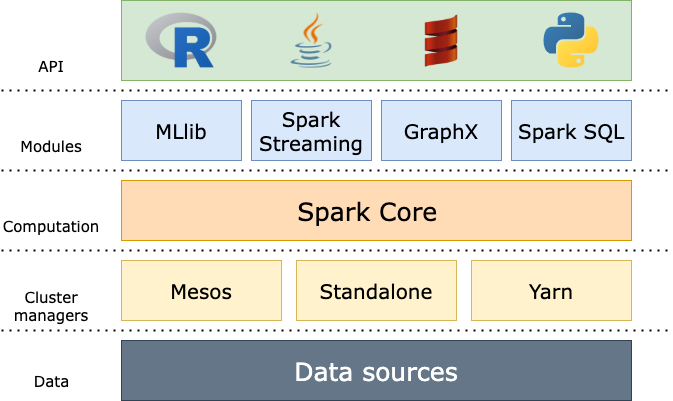
\includegraphics[width=0.8\textwidth]{obrazky-figures/ecosystem.drawio.png}
\caption{Unified stack of Apache Spark}
\end{figure}


\label{sec:rdd}
\section{Resilient distributed datasets }

Spark achieves its high speed by using a data abstraction called Resilient Distributed Dataset. They can be described as read-only collections of objects with assured fault-tolerant parallel processing, hence the name RDD. They were first introduced in the paper \cite{rdds}. 
Let us go over these features in more detail \cite{githubbook}:


\begin{itemize}
\item \textbf{Resilient} - fault-tolerant, RDD can be recalculated after a fault of a node or when a partition is missing. That is possible because a lineage graph of all operations is kept.
\item\textbf{Distributed} - data reside on several nodes of a cluster
\item\textbf{Dataset} - collections of data with primitive or structured values that represent records of the data you work with.
\item\textbf{In-Memory} - as previously mentioned, Spark calculates and holds data in memory to make the processing faster. It tries to keep as much data and as long as possible to optimize time and size.
\item\textbf{Immutable} - RDDs are read-only structures.  That means they do not change after they are created. After using a transformation on RDD a new RDD is created.
\item\textbf{Lazy evaluated} - another feature that can optimize the calculation is lazy evaluation. It means RDD is only calculated after an action prompts the execution. That means that multiple transformations might be chained before the evaluation.
\item\textbf{Cacheable} - even though Spark uses in-memory computations, it is still possible to~hold data in persistent storage.
\item\textbf{Parallel} - since the data is distributed across the cluster, parallel processing is possible.
\item\textbf{Typed} - RDD records have types - primitive, e.g., Int, String, or structured, e.g., tuples (Int, String) or objects.
\item\textbf{Partitioned and Location-Stickiness} - records of RDD are split into logical partitions and distributed across the cluster. One can also define placement preference for RDD.
\end{itemize}



Users can manipulate RDD with two types of operations. Let us describe them in more detail.

\begin{itemize}
\item \textbf{Actions} - unlike transformations, action calls do not return another RDD. Actions start the worker nodes' evaluation of the chain of transformations. Actions results are sent back to the driver node. Examples of these operations are count, reduce, foreach, and others.
Actions can also save the result to data storage instead of sending it back to the driver node, such as the saveAsTextFile function.


\item \textbf{Transformations} - operations applied on existing RDD that create new RDDs. DAGs that are later optimized consist of a chain of these operations. Transformations use lazy evaluation, and two types of transformations exist.
\end{itemize}
Transformations can be described as having either narrow or wide dependencies. The two types of transformations are illustrated on \ref{fig:rdd-types}

Any transformation that can be evaluated from a single partition as input is narrow. \textit{Narrow transformation} is computed on a single partition of RDD without the need for~knowledge of the other partitions - without any exchange of data between nodes.
Some examples of these transformations are \texttt{map}, \texttt{filter}, \texttt{union}, or \texttt{flatMap}.

The second type is so-called \textit{wide transformation}. Computing this transformation will collect data from multiple nodes, process it, and shuffle it. This transformation can lead to~repartitioning of data and even a change in the number of partitions.
These operations are time-consuming since a ton of data has to move around.
Examples of these operations are \texttt{groupBy} or \texttt{orderBy}.


\begin{figure}[H]
    \centering
    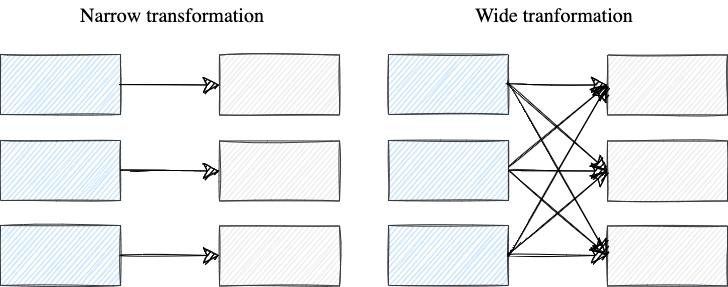
\includegraphics[width=0.8\textwidth]{obrazky-figures/rdd-types.drawio.png}
    \caption{Two types of RDD transformations}
    \label{fig:rdd-types}
\end{figure}
\pagebreak

\subsection*{DataFrame and Dataset}

With the development of Spark and its module came a need and a possibility to create new data abstractions. A new data structure abstraction called \textit{DataFrame} has been introduced in the Spark version 1.3 release. A few versions later, specifically 1.6, the next abstraction was added called \textit{Dataset}. In the major version of Spark 2.0, these were merged \cite{taleofthree}. DataFrame is only an alias for \texttt{Dataset[Row]} in Scala programming language or \texttt{Dataset<Row>} in Java. That means it is Dataset with the type \texttt{Row}. These data structures are heavily tied to the Spark SQL module. 

\subsection*{DataFrame}

DataFrame takes features from both RDD and relational database tables. That makes it immutable, distributed, fault-tolerant, and structured in columns and rows. 
They were designed to make data processing easier with higher-level structured abstraction. In addition, providing SQL-like language to manipulate the data makes it possible for a wider audience of developers. 

\subsection*{Dataset}

Datasets are the newest data structure in the Spark ecosystem. 
It provides benefits of both RDDs (strongly typed, lambda functions) and Spark SQL's execution engine. Even though the Dataset API is available only in Scala and Java, Python and R are still able to utilize multiple benefits due to their dynamic nature.


Let us take a look at why merging Dataset and DataFrame APIs was beneficial.

\begin{itemize}
\item \textbf{Static typing}- Syntax and semantic analysis are already being checked at compilation which prevents possible run-time errors.
\item \textbf{Highly abstract data structure} - as I already mentioned, DataFrame is an alias for \texttt{Dataset[Row]}. That makes the data highly structured with the possibility to map it to a user-defined class in a supported language.
\item \textbf{Ease of use} - the API offers functions similar to SQL aggregation operations. It may lead to a reduced number of operations from the use of RDDs.
\item \textbf{Performance} - Spark SQL uses an optimizer called Catalyst. Thanks to this optimization, using DataFrames can lead to better performance than RDDs which do not use any built-in optimizer. The part of Catalyst is the Tungsten memory manager. Tungsten converts data to binary form that takes up less memory than serialized data.
\end{itemize}


\section{Example of Spark code in Scala}

Finally, let us look at some code snippets of the Spark framework in Scala. These snippets will be helpful when discussing the code generation of the Spark application.

I already mentioned that a new RDD is created after using a transformation on an~already existing RDD. There must be a way to create RDD from pure data. Listing \ref{lst:parallelize} shows how new RDD can be created in Scala. The usage of transformation and action operations are displayed on listing \ref{lst:transact}. Finally, usage of Dataset and conversion back to RDD is shown in listing \ref{lst:dsrdd} taken from \cite{sparkdataset}.

\begin{lstlisting}[style=myScalastyle, caption={How to create new RDD}, label={lst:parallelize}]
    // sc - SparkContext
    // create rdd using parallelize
    val rdd1 = sc.parallelize(1 until 10)
    // create rdd from file
    val rdd2 = sc.textFile("/path/to/data/file.txt")
\end{lstlisting}



\begin{lstlisting}[style=myScalastyle, caption={Usage of transformation and action on RDD}, label={lst:transact}]
    // sc - SparkContext
    // transformation of previously created rdd
    val odd = rdd.filter(x => x%2 == 1)
    // action does not return new rdd
    odd.foreach(println)
    // prints out: (the order is random because RDD is distributed)
    // 1
    // 7
    // 9
    // 3
    // 5
\end{lstlisting}
\begin{lstlisting}[style=myScalastyle, caption={Usage of Dataset}, label={lst:dsrdd}]
    val linesDS = sc.parallelize(Seq("Spark is fast", "Spark has Dataset", "Spark Dataset is typesafe")).toDS()
    val words = linesDS.flatMap(_.toLowerCase.split(" ")).filter(_ != "")
    val groupedDS = words.groupBy("value")
    val countsDS = groupedDS.count()
    countsDS.show()
    val rddFromDS = countsDS.rdd
    // +--------+-----+
    // |   value|count|
    // +--------+-----+
    // |    fast|    1|
    // |      is|    2|
    // |   spark|    3|
    // | dataset|    2|
    // |     has|    1|
    // |typesafe|    1|
    // +--------+-----+
\end{lstlisting}


\chapter{Model-driven Development}
\label{chap:mdd}
Model-driven Development is a methodology of building complex software with the use of~simplified abstractions of already existing components. The main idea is to move the~development to a higher level of abstraction that is later used to generate the source code.   These components are visual building blocks that show the application and the business needs instead of looking through complicated lines of code. MDD helps bridge the gap between developers and business domain experts. 

Model is the fundamental part of the MDD paradigm. It defines the behavior, structure, and functionality of a system or a part of it. The MDD approach focuses on the construction of a visual representation of a software model. The model specifies how the system works and is used to generate the necessary code.

MDD methodology claims to have multiple advantages:

\begin{itemize}
    \item It increases developers' productivity because most of the code is generated from the~model or its components.
    \item The fact that MDD increases the system's abstraction level makes the communication between developers and other business experts easier. Business experts often do not understand the complex code but can communicate their ideas to developers using a~simple graphical representation.
    \item Since the code is generated, it becomes more consistent across the codebase because of reusable components.
    \item With enough support for code generation, modeling a system is independent of the~underlying technology.
\end{itemize}


In any technical decision, there always comes a trade-off. So let us mention some flaws that might hold MDD back.

\begin{itemize}
\item The complexity of some artifacts might be too high to model properly with abstract modeling. That may lead to manually editing the generated code, creating inconsistencies across the codebase.
\item The usage of models or UML is very different across the developers. Some may sketch the model to get the idea across. Others might use it to design the software, later coded by the developers. These two approaches differ from the MDD methodology of~using modeling as a programming language.

\item To create proper code generation tools, most of the MDD notations need to be standardized.
\end{itemize}
There are still a few things a developer could question, such as performance, maintainability, or scalability. Performance could be compared to traditional compilers, where it took a~long time and effort to create optimal compilers, while MDD is still a developing concept. Maintainability comes from the usage of MDD. If the developer changes the code without reflecting the change in the model, they can introduce many inconsistencies. This problem could be solved with a reverse code generation to regenerate the graphical model from code.
Finally, scaling is the biggest advantage MDD offers. Providing a higher level of abstraction to a system worked on by hundreds of developers can hold the generated codebase and diagrams more consistent across the company \cite{pragma-mdd}.


\subsection*{Model-driven architecture}

MDA is an approach to software design, development, and implementation introduced by The Object Management Group \footnote{https://www.omg.org/}. MDA offers guidelines for structuring software represented by models. It separates the business and application logic from the underlying platform. That means platform-independent models of applications or systems can be realized on virtually any platform. It also means the separation of the two that creates a~possibility for each to develop at their own pace. The business quickly responds to business needs, and the technology improves with the new development \cite{mda}.







\section{UML - Unified Modeling Language}
The Unified Modeling Language is a formally defined and standardized modeling language to specify, design, and document software systems (or other systems). It is a programming language independent. UML is widely known and used to model systems, especially object-oriented software. 

There are three common ways people use UML \cite{learningUML}:
\begin{itemize}
    \item \textbf{as a sketch} - usually by hand without the need of modeling tools
    \item \textbf{as a blueprint} - with the use of modeling software to generate parts of the source code
    \item \textbf{as a programming language} - the model is designed so it can run without any other interaction
\end{itemize}

In UML, we want to work with the abstraction of reality, and with different language means, we create the abstraction of the system - the model. In this model, we try to~capture relationships between different elements of the designed system. As the systems we try to~design can be pretty complex, we need to use multiple types of diagrams. Therefore, UML offers several types of diagrams that can be categorized into views. This categorization helps capture only the relevant parts for the modeling and ignore the others. 

The set of views that is known as the 4+1 Views of Software Architecture(see figure \ref{fig:views}) with examples of a diagram is as follows \cite{vpuml}:

\pagebreak

\begin{itemize}
\item \textbf{logical view} - an abstract description of the structure of units of implementations; modeling of its components and relationships(class diagram, sequence diagram)
\item \textbf{process view}  - the model of system behavior (activity diagram)
\item \textbf{deployment view}  - model the components required for deploying the system (deployment diagram)
\item \textbf{implementation view}  - describes how components are organized in packages and modules (component diagram)
\item \textbf{use case view}  - captures the user requirements of a system (use case diagram)
\end{itemize}

\begin{figure}[H]
    \centering
    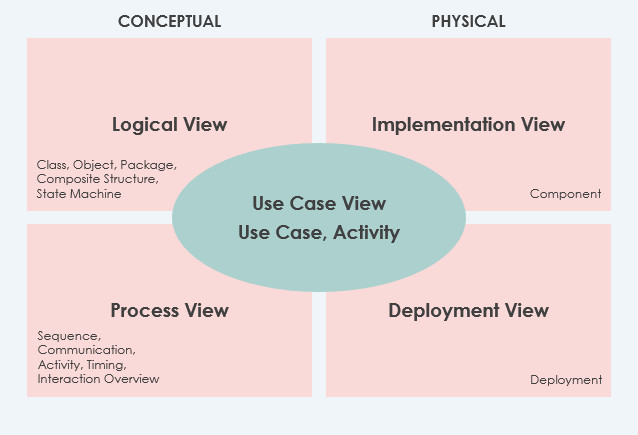
\includegraphics[width=0.8\textwidth]{obrazky-figures/modeling-structure-views-using-uml.png}
    \caption{UML views}
    \label{fig:views}
\end{figure}

\section{UML profile}

UML, on its own, is a very generic modeling tool. However, when a developer wants to~model a domain-specific problem, the standard UML might not be sufficient. The need for~an~extension of UML that would specify the domain-related problem made the OMG consortium include an extension mechanism called UML profile \cite{dip-umlprofile}. Profile package included in UML provides the means to extend UML meta-classes that still follow the UML standard. The usage of profiles can lead to adjusted UML for a specific domain problem. That means the code generators for a specific domain can be developed easier.
This technique is not used to create a new type of diagram; instead it extends an already existing type. Most UML editing software (CASE - Computer-Aided Software Engineering) supports the creation and usage of profiles because they only graphically extend elements of~already existing and well-known diagrams.

To define UML profile we use three standard elements as defined in \cite{learningUML}:

\subsection*{Stereotypes} 
Stereotypes signify that an element has a particular use or intent. Stereotypes are most often shown by specifying the name of the stereotype between two guillemots - \texttt{«stereotype»}. The number of stereotypes an element can be extended by is not limited. In that case, they are separated by a comma: \texttt{«stereotype1», «stereotype2»}. 
As shown in figure \ref{fig:stereotype}, while modeling Java classes, we can define stereotypes such as Entity Bean and Session Bean that inherit from the Bean stereotype. 
Other well-known stereotypes often used in~the~use-case diagram are \texttt{«include»} and \texttt{«extend»}.



\subsection*{Tagged values}

Tagged values are tied to stereotypes. A stereotype may have multiple tagged values associated with it. A piece of extra information is provided in a key-value manner. Figure \ref{fig:tagged} shows how tagged values are graphically represented. They can also be displayed in~a~note attached to the stereotyped element. As stated, tagged values are used to extend the properties of UML and are most commonly used for code generation, version control, configuration management, or authorship. 

\subsection*{Constraints}

Although stereotypes and tagged values are graphically represented in a diagram, constraints are not. Constraints impose rules and restrictions on model elements.
Constraints can be defined in informal language or using OCL - Object Constraint Language. Most diagram editing software supports this language and can check the validity of the diagram based on these constraints.

\begin{figure}[H]
    \centering
    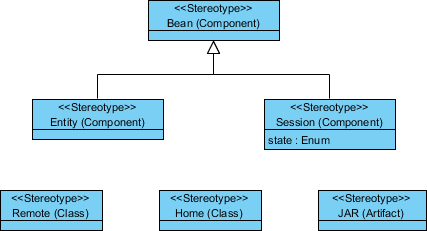
\includegraphics[width=0.7\textwidth]{obrazky-figures/05-ejb-profile.png}
    \caption{Example of stereotype}
    \label{fig:stereotype}
\end{figure}

\begin{figure}[H]
    \centering
    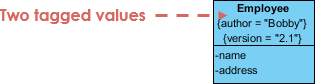
\includegraphics[width=0.6\textwidth]{obrazky-figures/02-class-with-tagged-value.png}
    \caption{Example of tagged values}
    \label{fig:tagged}
\end{figure}


\section{Eclipse Papyrus}

Eclipse Papyrus is an open-source graphical editing tool for UML 2 as defined by OMG. Eclipse Papyrus targets to implement 100\% of the OMG specification. It provides an~editor for almost all UML diagrams and supports UML profiles \cite{papyrus}. Papyrus also provides complete support to SysML to enable model-based system engineering. It includes an~implementation of the SysML static profile and the specific graphical editors required for~SysML. Papyrus is an excellent addition to the Acceleo workflow and Eclipse ecosystem overall.

\section{Eclipse Acceleo}

Eclipse Acceleo is a code generator implementing the Model-to-text specification \cite{mofm2t} defined by OMG. Acceleo lives in the Eclipse ecosystem, which is rich in modeling features. Acceleo is not only a code generator but has many features to extend Eclipse IDE with helpful tooling. Acceleo can generate any kind of code with its MTL (Model to Text) language that is compatible with any EMF-based model (Eclipse Modeling Framework) such as UML or SysML. The code generation language uses a template-based approach. A template is a~text containing dedicated parts where the resulting code is then calculated from the~input model. The dedicated parts are expressions specified on the element of the input model to~extract pieces of information defined in it. Acceleo uses OCL (Object Constraint Language) to~extract these pieces of information.

Acceleo supports incremental generation. This feature allows people to modify pieces of~generated code without losing these modifications when the code is regenerated, allowing the usage of generators to be more flexible. These areas are defined using the \texttt{[protected]} tag.



Acceleo is written in Java and is deployed as an Eclipse plugin and integrated into the Eclipse IDE. This plugin also brings multiple tools for the development of an Acceleo generator, such as an editor with syntax highlighting, auto-completion, error detection, a~debugger to check the state of generation step by step, and a profiler.

Since only running an Acceleo generator using Eclipse IDE is not optimal, Acceleo can also be used as a stand-alone application. The parsing and the generation engine are generated as a Java class that allows an Acceleo generator to be programmatically integrated into any Java application.

\begin{figure}[H]
\centering  
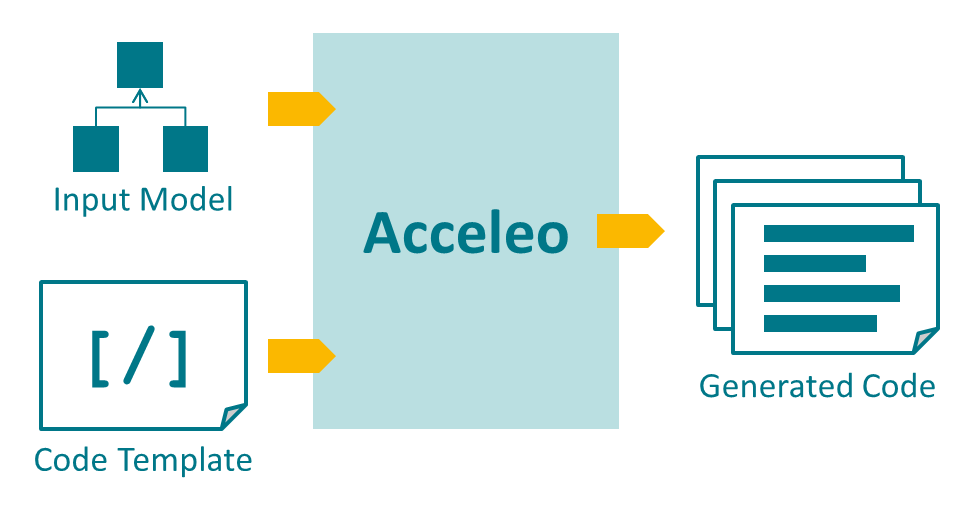
\includegraphics[width=0.50\textwidth]{obrazky-figures/acceleo.png}
\caption{Eclipse Acceleo \protect\footnotemark }
\end{figure}

\footnotetext{https://www.eclipse.org/acceleo/overview.html}

\subsection*{Java services}

Using OCL inside \texttt{[query]} construct in Acceleo might not always be enough to extract or modify the relevant information. Therefore, Acceleo offers an option to invoke Java code inside an Acceleo template. These services allow developers generate even the most complex requests. In order to use a Java service, use the Acceleo \texttt{invoke} operation in~order to~tell Acceleo to call your Java method and return the result. Java services are limited to~parameters and return values with a type from one of the meta-models used in~the~generator or a primitive type (String, Integer, Real, Boolean, etc.).


\chapter{Related work}
\label{chap:existing}

With the continuous rise of MDD several other projects with a similar goal in mind have been developed. The goal of this thesis is to design and implement a model-driven tool to~create Spark applications. By closely inspecting already existing solutions we can pinpoint the advantages and disadvantages of the given solution. 



\section{Executable UML}

First described in a book Executable UML: A Foundation for Model-Driven Architecture \cite{xuml}. Both a method and language to develop software, Executable UML (xUML) offers highly abstract and platform independent solution to generate source code from defined model. Even though xUML is a subset of Unified Modelling Language - UML, it uses slightly different semantics. The model does not include any code, but parts of the model are mapped to specific code snippets for target platform. Executable UML is a perfect example of Model-driven architecture in practice. 

\section{Map Reduce generator}

With the rise of the need for Big Data processing applications the field also tries to develop tools to make the analytic work more straightforward. The first proof of concept for Model-driven Development of Big Data processing applications was published in \cite{mdd-mapreduce}. Designing a meta-model for Map Reduce applications and subsequently generating a working source code proved that a Model-driven approach could be applied to processing tasks to bridge the~gap between developers and complex systems by abstraction. Even though this project uses a Map Reduce approach to data processing it still brings valuable insight into how Spark application can be modeled. The conclusion of this paper showed that MDD approach increased the productivity without any noticable performance overhead. 


\section{The custom Spark generator}

This project was developed as a master thesis \cite{dip-mddspark} with a similar goal. The meta-model of~this solution does not follow any standard. That makes it harder to learn. Even though the solution works, the modeling approach is quite complex. Using this meta-model you could model very complex applications as it is quite similar to modeling a Scala program by~assigning variables, calling and defining a function, and determining the order of execution.
The takeaway from this solution is the need for a meta-model to design the application with a much less complex diagram by trying to reduce the modeling space of an application. Also, the new meta-model has to use standard modeling language instead of a custom one, to make it easily integrable to Acceleo. 

\section{StreamGEN}

A very robust solution described in paper \cite{streamgen}. They developed a system with a similar approach and technical stack using UML profile and Eclipse Acceleo. StreamGEN is a system to generate Streaming Applications to multiple platforms - Apache Flink and Apache Spark. StreamGEN consists of a modeling language - StreamUML and an Acceleo code generator - StreamCGM. The meta-model is defined using UML profile to extend the Class diagram and the Composite Structure diagram. 
The authors decided to generate the application source code as Java code because it is widely supported by different platforms.  Since this solution is mainly focused on streaming applications it defines multiple domain-specific stereotypes such as a \textbf{WindowTransformer}, \textbf{WindowedStream}, or \textbf{RandomlyPartitionedStream}. Because the meta-model mainly focuses on stream processing some features are missing


\chapter{Meta-model design}
\label{chap:design}

In this chapter, I will introduce the designed meta-model that can be used to create a model of Big Data processing in Spark. I will describe its usage, advantages and disadvantages, and thought processes behind the design. 

As the previous chapter indicates I decided to extend the existing UML diagram with UML profile to add vocabulary to already existing, well-known language. UML and various domain-specific stereotypes are well known and have great support for both modeling and code generation - especially Eclipse Acceleo. 
To keep the trend of well-known principles I decided to extend the most common UML diagram - the Class diagram. 

The advantages of this approach are extensibility, reusability, and ease of use. The~class diagram can be easily extended with different profiles and used by different generators to create a more robust solution. The class diagram is also well known and more easily read than code. Finally, as stated in the previous chapter the Model-driven design makes diagrams reusable solutions as they can easily model parts of the system.

The proposed design also brings a few disadvantages. The designer needs to understand the Spark framework and Scala programming language. It does not abstract the~internals enough to seamlessly work without a prior knowledge of Spark. Also, the more advanced features of Spark are unable to be modeled (Streaming, MLlib) as their workflow is structured differently than the generic Spark processing pipeline.

This design is mostly inspired by the related work \cite{streamgen}, that was mentioned earlier. They took a similar approach by extending both the Class diagram and the Composite Structure diagram. Although this approach can bring better and more robust abstraction, I find using only one diagram more maintainable and reusable. This can bring a few hurdles that I will discuss later.


Now let us take a look at a Domain model of a typical Spark application. As we can see in figure \ref{fig:domain-model}, a Spark application structure is rather simple. An instance of Spark application has its own configuration. Most Spark applications use the command-line interface with provided arguments for control. After the Spark application is configured the~flow of~the~program can be represented as a directed acyclic graph. This is similar to how Spark actually works on the inside. These processing graphs begin with the source node. Afterward,  multiple transformations can chain to modify the input data provided by the~source node. The last type of processing node is the action node. Action node represents an action on computed RDD (or Dataset). 


\begin{figure}[H]
\centering  
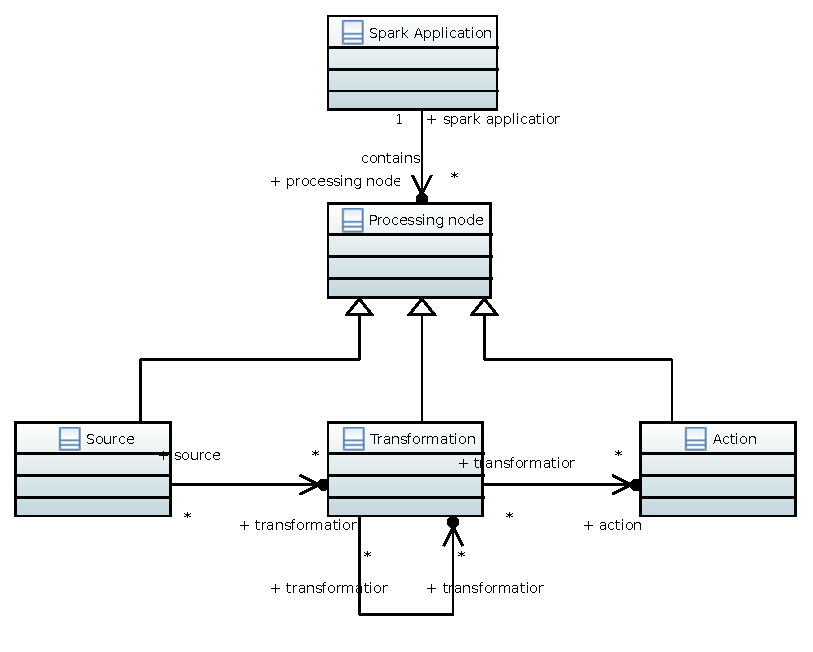
\includegraphics[width=0.75\textwidth]{obrazky-figures/Class_Diagram_0.pdf}
\label{fig:domain-model}
\caption{Domain model of Spark Application}
\end{figure}


Up until now, the order of generated code did not matter because the RDDs or transformation nodes were not evaluated. If the respective transformations were chained correctly the flow of the program was apparent. The problem arises when a single Spark application uses multiple actions. Their order must be deterministic because a premature action can modify the not yet evaluated source. That can be avoided by explicitly selecting the priority of a specific action.




With this domain model in mind I will define the meta-model in more detail. Figure \ref{fig:spark-profile} and table \ref{tab:table-name} show the designed UML profile. As already mentioned UML profile extends the most common diagram - the Class diagram. The most important types of elements of a UML diagram, or more specifically the Class diagram, are relationships (meta-class Association) and classifiers (meta-class Class). The meta-model also extends a less known meta-classes - Model and Datatype, to display the model with a better composition and provide a tuple data structure often used in Spark. 

\section{Description of provided stereotypes}

In this section I will describe the designed profile diagram and defined stereotypes in detail. 
It is necessary to mention the designed meta-model is designed with the Scala programming language in mind. Many tagged values of stereotypes require the user to specify Scala code snippets to define a function or an array of some sort. 


First I will describe miscellaneous elements that diagram provides. These elements all contribute to the type system of the meta-model. The \texttt{Snippet} primitive is defined to~distinguish the fields that expect String primitive or Scala code snippet to be provided. The~structered DataTypes \texttt{Option} and \texttt{Program Argument} are defined as types used in~the~meta-model to introduce structured tagged values. \texttt{Option} is key-value map where key is a~string literal and value is a Scala code snippet (either a string literal in quotation marks or a variable name). \texttt{Program Argument} defines Spark Application program arguments, their data types and default values. Enumaration File Source Type narrows down the values for \texttt{«File Source»} stereotype. 


\begin{itemize}
\item \texttt{«Spark Application»} - this model stereotype defines Spark Application as a whole. Spark applications usually need a configuration. The most common attribute - \texttt{master} is defined as an explicit tagged value. Next tagged value is \texttt{conf}. \texttt{Conf} uses the~defined \texttt{Option} type to configure the Spark object using key-value pair configuration. Similiarly \texttt{arguments} define input arguments for Spark Application and their default values. \texttt{Imports} is a list of packages to be imported into the Spark Application. Last, \texttt{initialCodeBlock} is used to inject specific code at the start of the generated application. 


\item \texttt{«Processing Node»} -  the processing of input with transformations and finally evaluating it with action is the core of Spark applications. The processing node stereotype is abstract and defines the processing graph node. Multiple stereotypes extend it.

\item \texttt{«Source»} - the entry point of the data processing. Source node represents the initial creation of RDD (or Dataset).
Tagged value \texttt{priority} is used to determine the~order of execution to prevent any undefined behaviour occuring.
Source stereotype is extended by specific ways of RDD creation.

\item \texttt{«RDD Parallelize»} - the most basic creation of RDD. The tagged value \texttt{array} represents a Scala code snippet of an array of data, for example - \texttt{array=\char`\"Seq(1,2,3)\char`\"}. 

\item \texttt{«File source»} - Spark supports multiple file types to load the data from. The~type of file can be selected using the tagged value \texttt{format} and the \texttt{File source types} enumeration.  The enumeration is used to limit the input scope. The path to the~input file is configured using the \texttt{filePath} tagged value. Similar to \texttt{conf} in Spark Application stereotype, file source can be configured with \texttt{options} tagged value. The~fact that Spark application can load both RDD and Dataset from files means it might be necessary to provide a data type for Dataset. 

\item \texttt{«SQL»} - represents the SQL query from the Spark SQL storage. Using the tagged value \texttt{query} to define an input query. Also uses \texttt{datatype} tagged value.

\item \texttt{«JDBC»} - the last supported data source is by loading data from a database. The \texttt{URL} tagged value is self-explanatory. The \texttt{options} and \texttt{datatype} work the same as in the~file source. The necessary options are also explicitly used as tagged values - \texttt{user}, \texttt{password}, \texttt{tableName}.


\item \texttt{«Transformation»} - transformation nodes are the central part of the processing graph. The designed meta-model supports both RDD and Dataset transformations that make this stereotype abstract. The tagged value that both transformations inherit is the \texttt{func} value. It is used to define the transformation provided by the Scala Spark API\footnote{https://spark.apache.org/docs/latest/api/scala/org/apache/spark/index.html}. For example, if we want to use the map function to double the~value of~records in RDD we would set the tagged value as follows: \texttt{func=\char`\"map(x => x*2)\char`\"}. 


\item \texttt{«RDD transformation»} - stereotype representing the RDD transformation. Doesn't contain any tagged values because it inherits \texttt{func} from abstract transformation.

\item \texttt{«Dataset Transformation»} - works similar to RDD transformation but for Dataset API. The purpose of this stereotype is to be able to tell the generator to convert the~RDD to Dataset.

\item \texttt{«Action»} - the next defined stereotype extending the Class meta-class represents the~last node of the graph - the Action. Actions' \texttt{func} values work the same way as in terms of transformations. Most of the action functions just return a value. \texttt{«RDD Action»} and \texttt{«Dataset Action»} stereotypes are also defined and work similarly to~transformation.

\item \texttt{«Code Block»} - even though Spark Application mostly consists of the previously mentioned processing graphs, there is still need of some utility code either to display or format outputs or assign values to variables. The tagged value \texttt{code} contains a Scala code snippet. The stereotype is also part of the processing graph and the~provided code is generated while traversing the graph. The output of the previous node is injected into the code using \texttt{\$out} variable.

\item \texttt{«Variable»} - in some specific cases we need to introduce a variable into our computation. We might need to iterate in a loop while joining constantly changing RDD with another RDD. Or we just want our mapper to use program arguments. The~need of this stereotype might be more apparent when I discuss it's usage in a later chapter. It is possible to store a specific output of a processing node by connecting this stereotype with Information Flow relationship to it. Tagged value \texttt{dataType} defines the dataType variable will hold and \texttt{isRDD} is a bool flag to tell the generator variable will contain RDD of the provided data type.

\item \texttt{«Flow»} - this stereotype extends Information Flow relationship and is used to increase the ability to define the order of execution and reuse already defined transformations. \texttt{Priority} is used when a transformation output is sent to multiple nodes. The generated code will traverse the graph in depth-first search manner. \texttt{Tag} helps to name a specific flow in the graph. It is only useful if a specific transformation has input from two different nodes. The output of this transformation for each of these nodes is accessed via the same tag. If the Information Flow relationship does not use this stereotype the priority is always considered to be traversed last. Also the graph is generated for each tag from the input flows. 

\item \texttt{«Argument»} - extends the association relationship. Some of the transformations provided in Spark API use another RDD/Dataset to process the input e.g. \texttt{zip}, \texttt{join} or \texttt{intersect}. This relationship helps to inject a \texttt{Variable} stereotype as a function argument to a transformation node.

\item \texttt{«Tuple»} - while working with RDDs in Spark one can use transformations, such as \texttt{groupByKey} or \texttt{reduceByKey}, that need tuples as their data type. This stereotype extends DataType meta-class making it possible to use it as a data type in model when necessary. 

\item \texttt{«Loop»} - similarly to \texttt{«Spark Application»} stereotype this stereotype also extends the Model meta-class to display a proper composition of the application. \texttt{«Iteration Loop»} and \texttt{«Conditional Loop»} stereotypes define the loop condition since this stereotype is abstract. Both \texttt{iterations} and \texttt{condition} tagged values are Scala code snippets and represent the behaviour of the loop.

\end{itemize}


\begin{figure}[H]
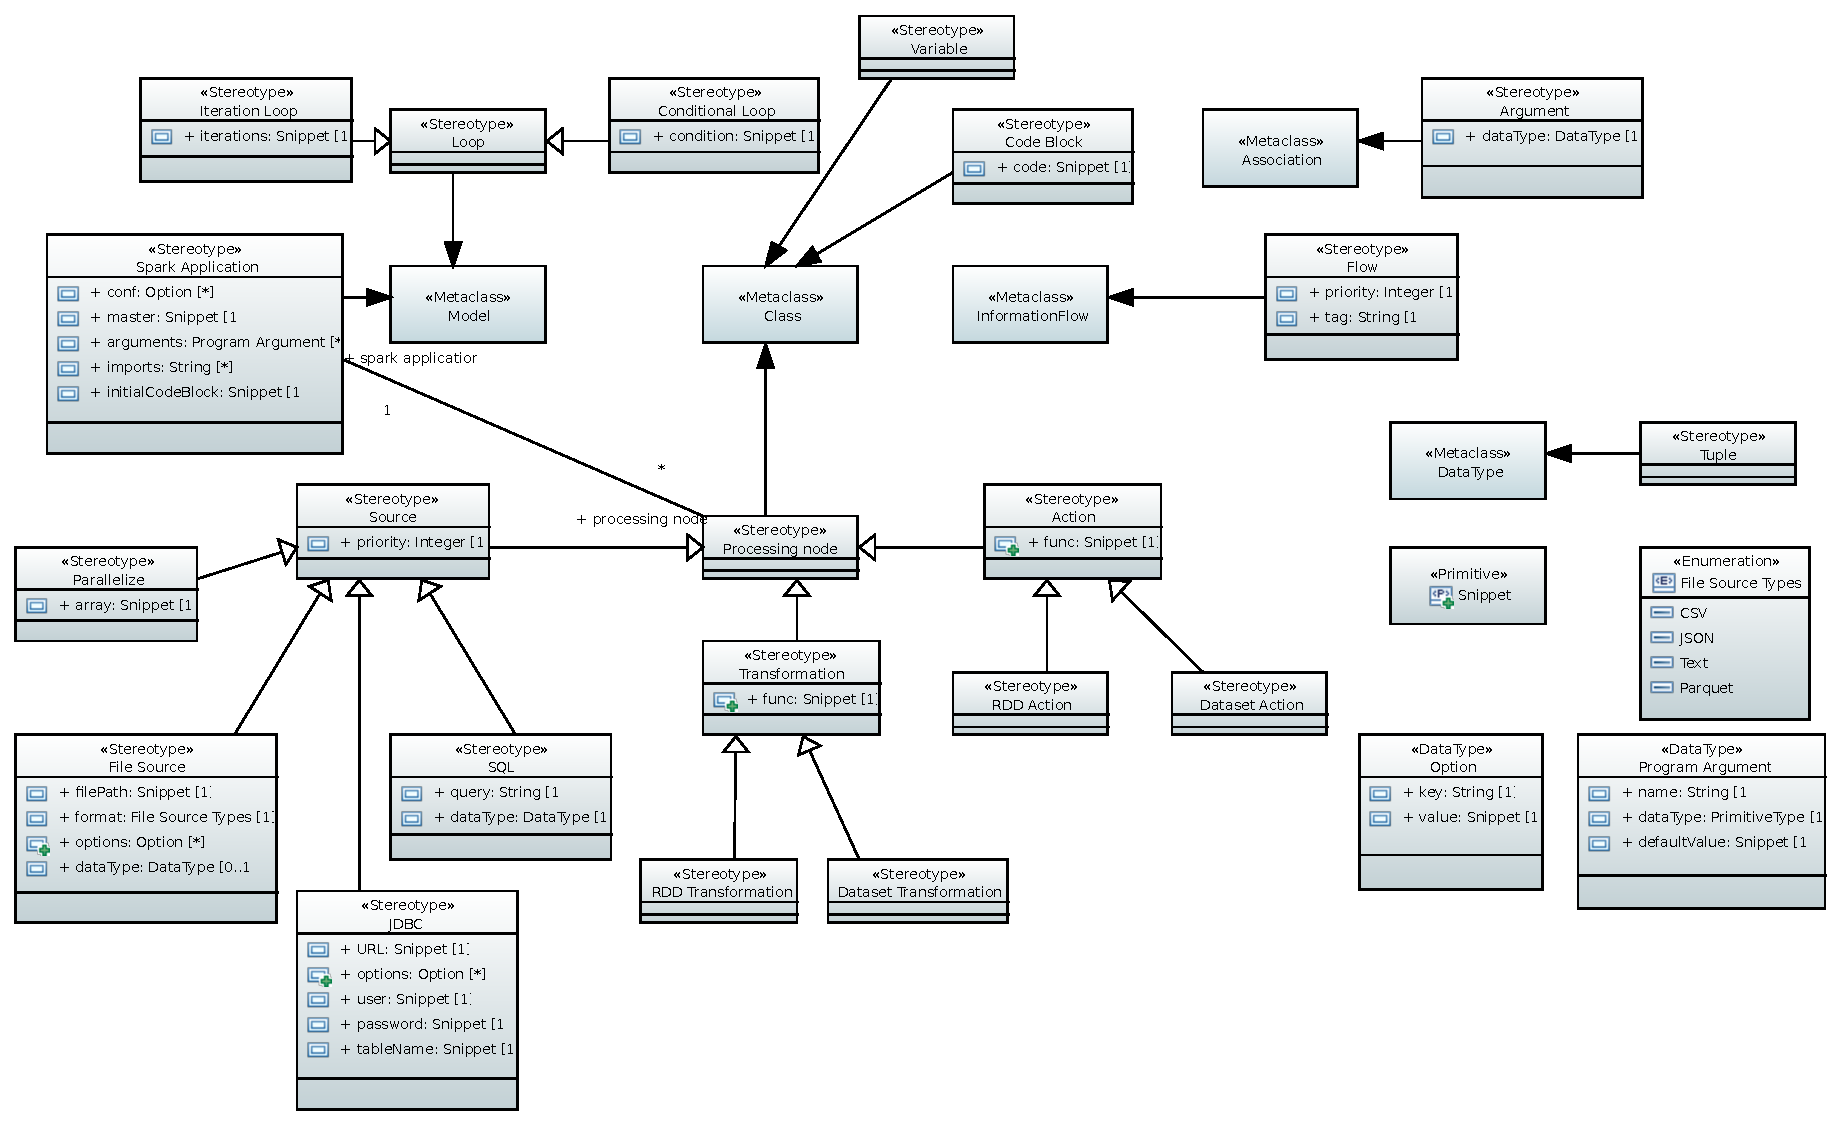
\includegraphics[angle=90,width=0.90\textwidth]{obrazky-figures/meta-model-diagram.pdf}
\label{fig:spark-profile}
\caption{UML Profile diagram describing Spark Application}
\centering
\end{figure}


\section{The usage of the profile}

There are a few non-standard design choices that need to be described to understand the~usage of the proposed meta-model. In this section I will go over the details that are necessary to understand to use the designed meta-model properly. 

\subsection*{Order of execution}

The source node and the action node can have multiple outputs and inputs respectively. The~transformation node can have both multiple inputs and outputs. This creates a situation where one diagram can define multiple processing pipelines. To determine which code is generated first, the source nodes and Information Flow relationships have priority values. The order of generation is as follows: 
\begin{enumerate}
    \item find the highest priority source node
    \item generate the code representing graphs in depth-first search manner where higher number has higher priority
    \item select next source node and repeat
\end{enumerate}

In many Spark Application the processing nodes might only contain one output. To~make the modeling process more straight-forward, even the Information Flow relationships without the \texttt{«Flow»} can be used to model the computation. These relationships are then considered to have the lowest priority when possible branching occurs.  

\subsection*{Data Types}

The graph, created using Information Flow relationships as edges and processing nodes as nodes, instantiates the processing pipeline of the application. Each edge must contain data type of the RDD that is being processed. This data type is selected using \textit{conveyed} property of the Information Flow relationship. 

To define data types used by different elements across the diagram, such as Information Flow relationships, variables, and sources, the package element of a Class diagram is used. If the package is contained inside the \texttt{«Spark Application»} stereotype model element, the~appropriate data structures are also created by the code generator. Class diagram offers primitive data types - Integer, Real, Boolean and String. It is also possible to modify the multiplicity of the attribute to create a list. Meta-model supports the definition of a~structure type with primitive data types and their multiplicity. The generated case classes and data types are later described in chapter \ref{chap:impl}. On the other hand, some data structures, or in this case Scala case classes, can include properties that can not be modeled in the UML Class diagram. The meta-model can still support these data types as an imported anonymous data type. To import the data types, use the \texttt{imports} tagged value of the~\texttt{«Spark Application»} stereotype. Afterward, create a package element with a DataType element inside. This element does not need to have any properties defined, but requires the~name to match the~imported name. The difference between imported and generated data type can be seen in figure \ref{fig:datatypes}.


\begin{figure}[H]
\centering
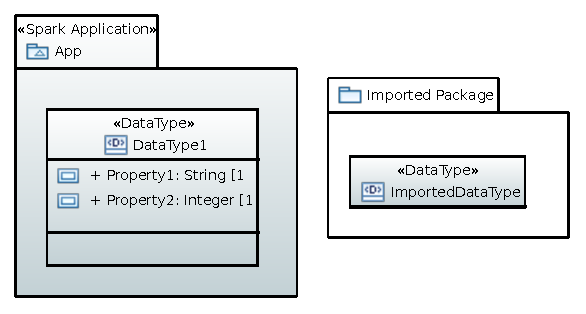
\includegraphics[width=0.7\textwidth]{obrazky-figures/package-example-diagram.pdf}
\label{fig:datatypes}
\caption{Difference between generated and imported data type}
\end{figure}


\subsection*{Loops}
The analyzed related projects did not include any form of loops in their design. Therefore, the addition of loops to the meta-model brought the possibility to model more complex applications. To properly include this feature, both the readability and functionality of~the~diagram must be considered. Similarly to the Application element, loops are also represented as the model element of the Class diagram. The model element can display what nodes of the computation are inside. Now it is crucial to determine when the loop scope starts and where it ends. As the generator traverses the computational graph, when the first node with a new loop scope is visited, the loop header will be generated. The~closure of~the~loop happens when the generator visits the first node outside of the model element.  The meta-model also supports nested loops and thanks to the model element the~diagram remains readable. 

\subsection*{Tags}

The meta-model is designed to be a Class diagram. Classes are not meant to represent objects already instantiated in the application. The overall thought behind the meta-model design is that the nodes represent the structure and the template of computations, while Information Flow relationships instantiate them inside the application's main method. Therefore, all the nodes inside the diagram must be unique. Tagged value \texttt{tag} in~the~\texttt{«Flow»} stereotype aims to prevent a definition of multiple classes with the same method, but different name. When the computation requires to process multiple inputs with the same function, it is possible to connect these inputs to a processing node. These input edges must then be distinguished by tagging them with a specific value. To differentiate between the~output flows, the same tag must be used in the out-coming relationship. If no tag is used in the output Information Flow relationship, all the inputs are processed and the~generator continues to generate the pipeline for each of them. It is important to mention that if only single Information Flow relationship is used it can only hold a single conveyed data type, whereas the inputs types to the processing node may differ.  The use of tags is shown in~the~Dataset processing test case described in the section \ref{sec:sqlprocess}.

\subsection*{Datasets}

When using Spark's Dataset API, it is often necessary to use the name of the input Dataset variable. An example can be seen in listing \ref{lst:this}. However, the name of the generated variable holding the value is unknown. Therefore it is necessary to provide this functionality to~the~model designer somehow. Test case \ref{sec:sqlprocess} shows the code snippet of the solution. Because outputs from all the nodes are cast to RDD, the transformation and action methods need to use API with the \texttt{\$} notation. The input Dataset is then renamed to \texttt{this} using an~alias method. 
\begin{lstlisting}[style=myScalastyle, caption={Dataset API using the name of Dataset variable}, label={lst:this}]
    people.filter("age > 30")
     .join(department, people("deptId") === department("id"))
     .groupBy(department("name"), "gender")
     .agg(avg(people("salary")), max(people("age")))
\end{lstlisting}


\subsection*{Variables}

Another fairly non-standard feature is the use of variables. This element defines a variable in the main method of the application. The name of the element matches the variable inside any Scala code snippets. The injected variable also uses the same identifier inside the transformation and action function. 


\vspace{20px}
\begin{table}[H]
\centering
\begin{tabular}{@{}lll@{}}
\toprule
Stereotype               & Inherits from      & Type     \\ \midrule
«Spark Application»      & Model              & Concrete \\
«Computation Node»       & Class              & Abstract \\
«Source»                 & «Computation Node» & Abstract \\
«File Source»            & «Source»           & Concrete \\
«SQL»                    & «Source»           & Concrete \\
«Parallelize»            & «Source»           & Concrete \\
«JDBC»                   & «Source»           & Concrete \\
«Transformation»         & «Computation Node» & Abstract \\
«RDD transformation»     & «Transformation»   & Concrete \\
«Dataset transformation» & «Transformation»   & Concrete \\
«Action»                 & «Computation Node» & Abstract \\
«RDD Action»             & «Action»           & Concrete \\
«Dataset Action»         & «Action»           & Concrete \\
«Flow»                   & «Information Flow» & Concrete \\
«Code Block»             & Class              & Concrete \\
«Variable»               & Class              & Concrete \\
«Tuple»                  & DataType           & Concrete \\
«Loop»                   & Model              & Abstract \\
«Iteration Loop»         & «Loop»             & Concrete \\
«Conditional Loop»       & «Loop»             & Concrete \\
«Argument»               & Association        & Concrete \\ \bottomrule
\end{tabular}
\caption{\label{tab:table-name}The list of defined stereotypes}
\end{table}




\chapter{Implementation details}
\label{chap:impl}
For this chapter, I will go over the implementation details of the Spark Application code generator. Both the meta-model definition and code generator are integrated into~the~Eclipse modeling ecosystem. Futhermore, both Papyrus and Acceleo follow OMG standards. Therefore the designed solution is technologically independent in theory. 

The code generator is implemented in Acceleo and can be divided into two parts. First, the generation of necessary Scala classes, and second, the generation of the computational graph. The implementation also contains two kinds of source files. Acceleo \texttt{.mtl} template files and Java services, both found in \texttt{src} folder. Java services are mostly used to generate the complex computational graph while templates are used to define the folder structure and class implementations. 

The final generated \textbf{main/scala/\{app\_name\}/} folder has the following structure: 
\begin{itemize}
    \item \textbf{actions/} - folder containing action classes
    \item \textbf{dataTypes/} - folder containing dataType case classes
    \item \textbf{sources/} - folder containing source classes
    \item \textbf{transformations/} - folder containing transformation classes
    \item \textbf{\{app\_name\}App.scala} - file with the application object and the main method
\end{itemize}

The generated folder structure represents the application source code. The best approach to folder structure is to include the generated folder in the \texttt{src/} folder of the project. The generator does not generate the whole project but only the needed source code.

\section{Scala classes}

The generator creates multiple classes. To make the model more extensible, each node of~the~computational graph is represented as a Scala class. Also, the data types defined in~the~model are generated as Scala case classes. Scala's case classes represent immutable data defined as a data structure with methods. A sample generated data type is shown in~listing \ref{lst:caseclass}. If the case class needs to be enriched with potential methods to modify data, the already mentioned \texttt{[protected]} tag is used and represented as a user code comment. This section can be modified and is not included in the model. This code block is not lost after a subsequent generation of the application if a change occurs. 

\begin{lstlisting}[style=myScalastyle, caption={The generated Counter class}, label={lst:caseclass}]
    case class WordCount(
    	var Word: String,
    	var Count: Long,
    ){
    //Start of user code WordCount
    //End of user code
    }
\end{lstlisting}


As per Scala's best practices, each class is generated into its own file. This approach to~class-based code generation is different than how most Spark Application code is written. I believe that this approach is more extensible and robust, even though it creates more boilerplate code. An example of a generated class can be seen on listing \ref{lst:wordSplitter}.

Multiple important details might be pointed out. The class consists of a single method and multiple properties. These properties do not influence the generated application in~any way. They serve to demonstrate the potential possibility of reverse model generation. In~the~future, a tool might be developed that would complement Acceleo's M2T generation by reversing it to Text to Model transformartion. By introducing these properties it is possible to define the stereotype and tagged values of a class. 

\begin{lstlisting}[style=myScalastyle, caption={The generated Counter class}, label={lst:wordSplitter}]
    class Counter() {
    	val S_rDDTransformation = true
    	val TV_func = """reduceByKey(_+_)"""
    	
    	def transform[T: TypeTag](rdd: RDD[T]) = {
    		typeOf[T] match {
    			case type1 if type1 =:= typeOf[(String, Long)] =>
    				rdd.asInstanceOf[RDD[(String, Long)]]
    					.reduceByKey(_+_)
    		}
    	}
    	//Start of user code Counter
    	//End of user code
    }
\end{lstlisting}

Every single computational node; source, transformation and action contain a single method - \texttt{source}, \texttt{transform} and \texttt{action} respectively. This method implements the logic provided by tagged value \texttt{func}. The method uses generic types and reflection because a~single transformation or action can have multiple inputs with different types. The use of reflection is closely described in section \ref{sec:reflection}. The use of~multiple data type inputs to~a~single processing node can be seen later in section \ref{sec:sqlprocess}. Both transformation nodes and action nodes extend RDD and Dataset operations. To abstract away the communication between them, every output is defined as \texttt{RDD[T]} of the specific type. This leads to the need of~re-typing RDD to Dataset using \texttt{toDS()} method, when Dataset action or transformation is used.

\section{Computational graph}

The more complex part of the code generation that creates the flow of the application is the~generation of the computational graph. Because of the complex nature most of the~generation is located in Java services. The implementation of the computation is located in the~main method of the App object. If the previous generated code was represented by classes of the model, this part is represented by Information Flow relationships that instantiate the classes and produce outputs. A few other necessary elements are also included in this part of the generation, namely loops, code blocks and variables. 

First, all necessary classes are instantiated. All nodes are stored in variables with a~specific name - prefix \texttt{S\_}, \texttt{T\_} and \texttt{A\_} and properly formatted name of the class in the~diagram. 
After that, the graph is traversed depth-first while creating necessary statements. The~output of each node is then stored in a variable with a similar name to the node it was produced by. Starting with prefix \texttt{s\_}, \texttt{t\_} and \texttt{a\_} and the name of the node, and ending with suffix \texttt{\_\{tag\_name\}}. The suffix is omitted if the particular flow does not contain any tag. 

\section{Loops}

Some Big Data processing tasks might include a specific loop to process data, e.g., tasks such as k-means clustering, linear regression, or page rank calculation (described in chapter \ref{chap:testing} in more detail). Including loops in the meta-model brought many hurdles implementation-wise. Since loops extend model, the graph node must have been searched for recursively in the application model. 

Looking at how the loop is structured in code, we can see it wraps statements inside it. To correctly generate the loop while traversing the graph, the header is generated before the node statement when the computation enters a new loop scope. The recursive traversal of the graph keeps track of the loops in the model and currently active loops - meaning loops where the end of the scope is yet to be generated. When processing a new node, the~generator checks the scopes it is inside of. If any active loops are missing, the proper loop scope is closed.

As previously mentioned, new variables are defined for each output of a node. Therefore, some of these variables can be defined inside the loop's scope. During the first prototyping of loop implementation, a problem arose when these variables needed to be accessed outside the loop's scope. This situation happens when the graph leaves the loop and uses the~output of the last node inside the loop. The implemented code generator handles the~problem by~defining the variables located inside the loop at the beginning of the graph. Only necessary variables are defined to lower the amount of generated boilerplate code. The~solution can be seen in a sample code snippet shown in listing \ref{lst:pagerankloop}. 

\section{Data Types}

Scala as a programming language is statically-typed. That means all necessary data types must be known during the compilation of a program. The fact that the generator creates much boilerplate code to make the model more extensible also removes the possibility of utilizing Scala's type inference feature. Also, the type system in UML modeling is fairly limited. As previously mentioned, it is only possible for a few primitive types, their multiplicity, or the user-defined structure of these primitives. The import and data type definition outside the model element feature attempts to include more complicated data types. These data types are then generated as \texttt{\{datatype\_name\}}. See the code snippet in~section \ref{sec:sqlprocess}.

It is necessary to mention the use of primitive types of the UML, especially \textit{Integer} and \textit{Real}. The internal conversion between Dataset and RDD using \texttt{toDS()} and \texttt{rdd} methods, introduces a possible typing problem. To prevent this \textit{Integer} is represented as \texttt{Long} data type in Scala and \textit{Real} is \texttt{Double}. This fact is also necessary to understand when modeling a Spark task using the meta-model. As seen in figure \ref{fig:wordcount}, the \textbf{CountAdder} class uses \texttt{1L} to define the number as \texttt{Long}. 


\section{Arguments, code blocks and variables}

Spark Applications might need to use other code than RDD actions and transformations. This issue is solved by including code blocks and variables. These parts of code are also considered to be processing nodes in the diagram. The generator first defines all variables in~diagram with their assigned data type and \texttt{null} value. If the variable is part of~the~computational graph connected by Information Flow relationship, then a re-assignment statement is generated as the variable is already defined. 

Code blocks nodes and \texttt{initialCodeBlock} tagged value are generated at appropriate places as Scala code snippets are used to introduce custom functionality or possibility to~model specific work-arounds. 

Finally, program arguments are generated as shown in listing \ref{lst:arguments}. They represent the~application input and can take value of any primitive data type. Futhermore, if a node needs to use it as an argument, simply define \texttt{«Variable»} stereotype with the same name. When the generator creates the variable definitions it omits the variables defined in program arguments, because the generated code would throw variable already defined error. 

\begin{lstlisting}[style=myScalastyle, caption={Generated program arguments}, label={lst:arguments}]
    var argMaster = if (args.length > 0) args(0).toString else "local[*]"
    var argInt = if (args.length > 1) args(1).toLong else 1
    var argReal = if (args.length > 2) args(2).toDouble else 1.1
    var argBool = if (args.length > 3) args(3).toBoolean else true
\end{lstlisting}


\section{Reflection}
\label{sec:reflection}
To fully utilize the advantages of model-driven development, we want to reuse already modeled processing nodes as much as possible. With the introduction of tags in the meta-model, it is possible to distinguish the incoming flows to a transformation or action. These flows might convey different data types while still being compatible with the node's function. To support this approach, the generated code uses type reflection and type assertion to limit the generated boilerplate code. 

Even though Scala programming language supports method overloading, it can only be used on types without type parameters. As we already know, the processing graph always produces \texttt{RDD[T]}. Therefore, type overloading would not work. The next Scala feature that enables this approach is compound types\footnote{\url{https://docs.scala-lang.org/tour/compound-types.html}}. Thanks to compound type a Scala method returns values that act as multiple types at once. To distinguish the proper type, the generator uses type casting with the method \texttt{asInstanceOf[T]} in the computational graph code. 
The section \ref{sec:sqlprocess} takes a closer look at the advantages and code snippets of this approach.


\chapter{Sample test cases}
\label{chap:testing}
This chapter will demonstrate the usage, discuss and evaluate the solution. I prepared multiple relevant test cases that display the general usage and some of the features and quality of life design choices in the meta-model. By showing these test cases, I intend to~demonstrate the advantages of the meta-model while also pointing out where the model-driven solution to Spark tasks might come short. The diagrams, model meta-files and the~generated sources, have also been submitted with this thesis for further inspection.  


\section{Word Count}

Word Count is considered to be the \textit{"Hello, World!"} program for Big Data processing. This application counts the amount of each word in an input text. The sample model is shown in figure \ref{fig:wordcount}. 


\begin{figure}[H]
\centering
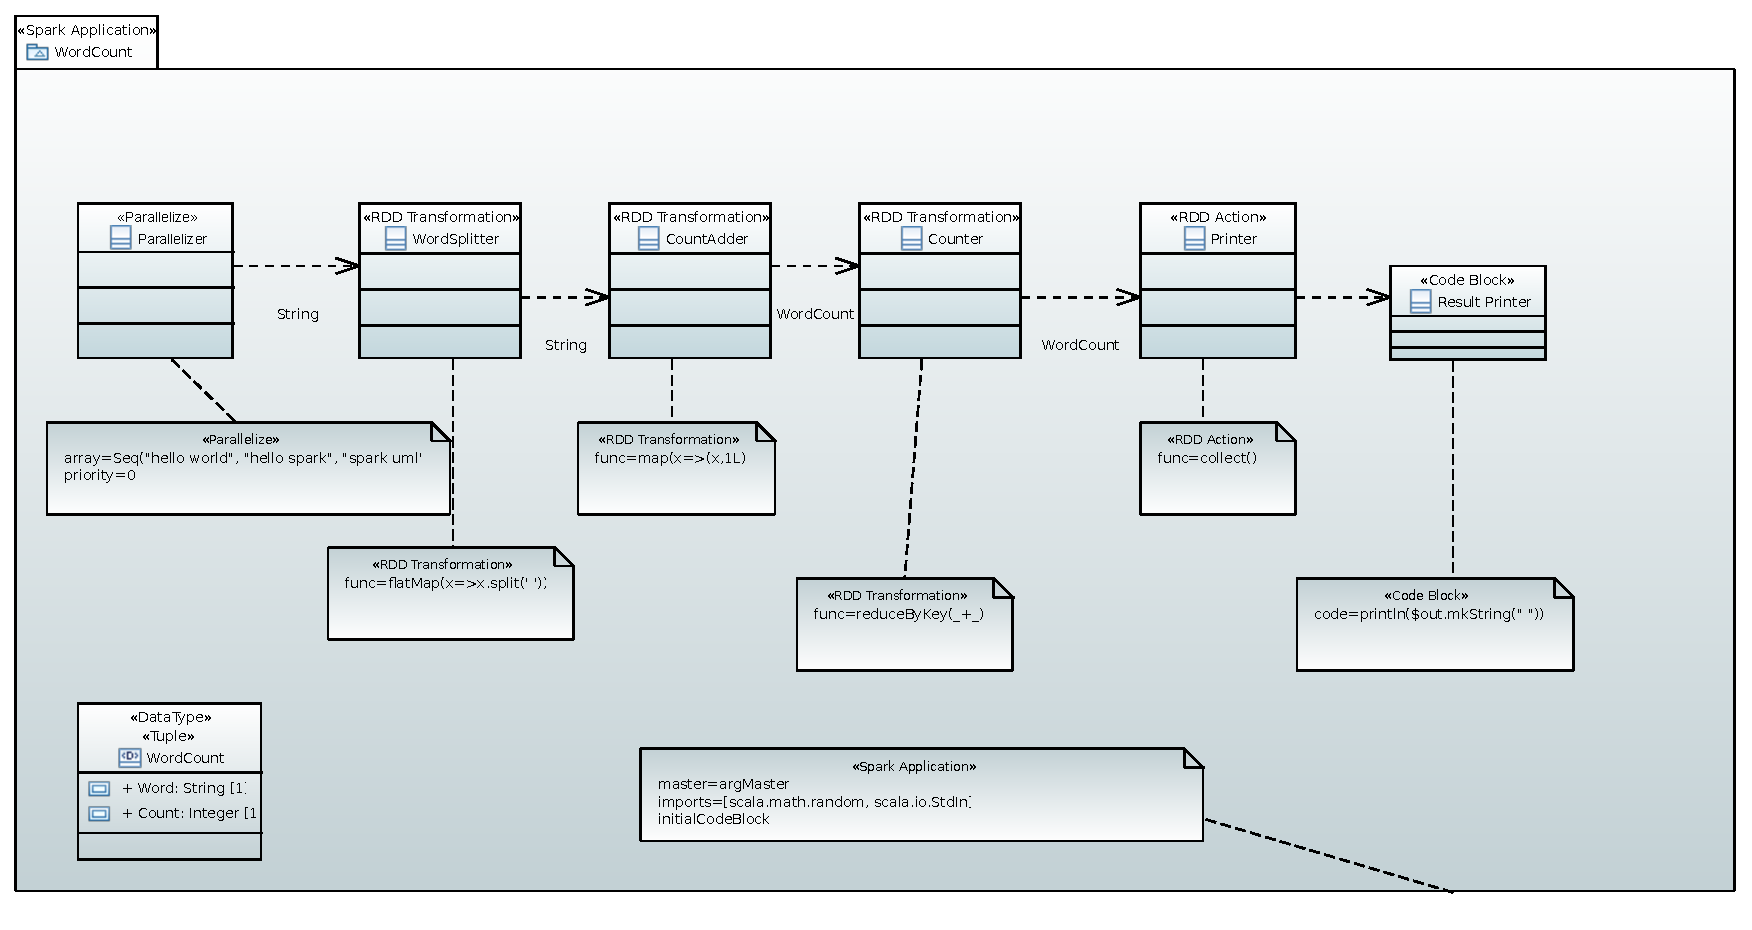
\includegraphics[width=1\textwidth]{obrazky-figures/word-count-diagram.pdf}
\label{fig:wordcount}
\caption{Word Count diagram}
\end{figure}

As seen in the figure, the diagram is a simple directed graph inside a model element. The~quick overview of the algorithm is quite simple. First, the input RDD is created. Although it is most often created from a text file, for demonstration purposes, the~\texttt{«Parallelize»} stereotype is used. Then, the input is split into RDD of strings of specific words using \texttt{flatMap}. After that, the Counter transformation processes the input to output defined key-value tuples. These tuples are then reduced by key to calculate the~occurrence of each word in the source text. Finally, the action node is used to collect the~desired result.

As we can see, the diagram uses the \texttt{«Tuple»} stereotype to introduce key-value pair data structure. Every Information Flow relationship conveys a specific data type, as previously discussed, these types represent the type of the RDD sent between two nodes of the graph (for example \texttt{RDD[(String, Long)]} for the tuple \textbf{WordCount}). The only Information Flow relationship without any data type is used when the graph finishes with the \texttt{«Code Block»} stereotype node. The output value from the previous node is accessed using \texttt{\$out} variable. The diagram also shows the need to use \texttt{Long} instead of \texttt{Integer} in the \textbf{Count Adder} class. 

As already stated, the generator creates a bunch of boilerplate code to make it more extensible or potentially introduce a possibility to support reverse model generation. Listing \ref{lst:wordcountcode} shows only the part of the main method, where the computation resides. 

\begin{lstlisting}[style=myScalastyle, caption={The generated Word Count computation}, label={lst:wordcountcode}]
	val s_parallelizer = 
	  S_parallelizer.source().asInstanceOf[RDD[String]];
	val t_wordSplitter = 
	  T_wordSplitter.transform(s_parallelizer).asInstanceOf[RDD[String]];
	val t_countAdder = 
	  T_countAdder.transform(t_wordSplitter).asInstanceOf[RDD[(String, Long)]];
	val t_counter = 
	  T_counter.transform(t_countAdder).asInstanceOf[RDD[(String, Long)]];
	val a_printer = A_printer.action(t_counter);
	println(a_printer.mkString(" "))
\end{lstlisting}

One may notice, that the generated computation seems very uniform and easy to read, that is because the code generator executes in the order of the computational graph. This uniform code also simplifies the potential reverse generation.

An argument can be had that this algorithm is only a simple sequence of steps without any complexity. However, the next test case introduces a more complex problem.



\section{Page Rank}

The next chosen test case is the Page Rank algorithm. Google Search uses this algorithm to~measure the~importance of a website page. Not only is this algorithm used with Big Data, but it also uses a loop. This fact makes it an excellent example to demonstrate the~usage of the designed meta-model. The integration into the Eclipse ecosystem that already has modeling features turns out to be a good choice for any modeling task. Papyrus offers the~possibility only to display the selected elements. As shown in figure \ref{fig:pagerank}, some of~the~elements are hidden, so the diagram is more readable while still holding the necessary information to generate the final application. Now let us look at some of the features used in this diagram. 

\begin{figure}[H]
\centering
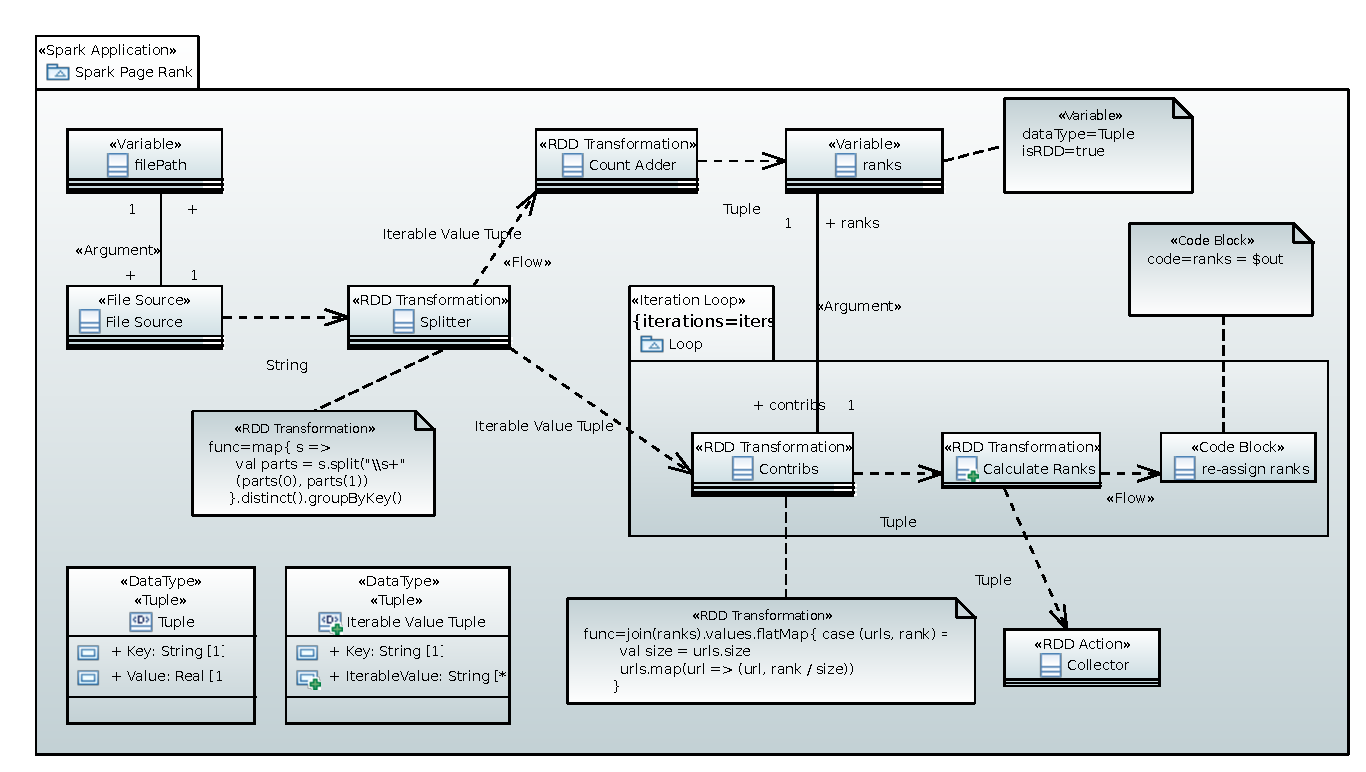
\includegraphics[angle=90,width=0.82\textwidth]{obrazky-figures/page-rank-diagram.pdf}
\label{fig:pagerank}
\caption{Page Rank diagram}
\end{figure}

First, we can see two tuples defined. The first defines a typical key-value pair already seen in the Word Count example. The second one differs in the multiplicity of the value element. This tuple is produced by the \texttt{groupByKey} operation. This tuple data type then represents \texttt{RDD[String, Iterable[String]]}.

Next, we can see that two nodes have multiple outputs. To determine the exact order of~the~execution, the \texttt{«Flow»} stereotype has been used for the higher priority path. As I already mentioned, Information Flows without the stereotype are evaluated last in an~undefined order. In this diagram, the generator first generates the path to the \textbf{ranks} node with the~\texttt{«Variable»} stereotype. This variable holds the output of the previous node. As can be seen in the diagram, the variable \textbf{ranks} data type is \texttt{RDD[(String, Double)]}. 

The computation node \textbf{Contribs} uses the previously defined variable in its
transformation. We can see the \texttt{«Argument»} stereotype being used to inject the variable into the~transformation. In a typical Spark application program, the transformation's anonymous function could reach out of its scope and use all variables defined in the app's main method. Since all nodes are generated as separate classes, all necessary variables must be provided to the method scope. This approach introduces more modeling work but increases the transparency of the used transformation and might also prevent bugs by using variables out of scope. An example of Linear Regression implementation with the transformation using variable out of the anonymous function scope can be seen in an official Spark example on GitHub\footnote{\url{https://github.com/apache/spark/blob/master/examples/src/main/scala/org/apache/spark/examples/SparkLR.scala}}. 

\subsection*{Loop}

Now let us discuss the loop. Listing \ref{lst:pagerankloop} shows the full generated computation of the~Page Rank diagram. The first thing to point out are the variable definitions for~the nodes inside the loop. If the variables were not defined before hand, the last statement in~the~listing would fail, because the \texttt{t\_calculateRanks} would only be defined in the scope of~the~loop.
The diagram shows that the path enters do loop when the \textbf{Splitter} node sends data to~the~\textbf{Contribs} node. Because of this transition, the appropriate loop header was generated. When the generator enters the \textbf{Collector} node, it closes the loop because the node is not inside the model element. 


The main reason to use a loop inside a Spark application is to modify inputs for~a~transformation. In this example, we need to modify the \textbf{ranks} variable in each iteration. If we tried to model the diagram differently, we might come across a problem. If the~\textbf{Calculate Ranks} tried to overwrite the data inside the variable node, it would exit the~model element, and the variable re-assignment would close the loop. Furthermore, if the~meta-model allowed to define multiple classes with the same name, it would disobey the~UML standard. That is why the variable re-assignment is modeled as the \texttt{«Code Block»} stereotype. This situation shows that the meta-model might be improved, but also that it is flexible enough to allow a specific program requirements to be modeled.

This test case aimed to present multiple features of the meta-model. The loops, the~function arguments, and the execution priority were proven to work correctly and offer a~relatively intuitive modeling experience. This example also highlights the advantages of this solution compared to already existing ones. Improving the ability to model more complex tasks while also keeping the graphical model readable is one of the~essential parts of~the~model-driven approach. The last example test case will go over the remaining features supported by the integrated meta-model.


\begin{lstlisting}[style=myScalastyle, caption={The Page Rank computation}, label={lst:pagerankloop}]
    var t_contribs: RDD[(String, Double)] = null
    var t_calculateRanks: RDD[(String, Double)] = null
    		
    
    val s_fileSource = S_fileSource.source(filePath).asInstanceOf[RDD[String]];
    val t_splitter = T_splitter.transform(s_fileSource).asInstanceOf[RDD[(String, Iterable[String])]];
    val t_countAdder = T_countAdder.transform(t_splitter).asInstanceOf[RDD[(String, Double)]];
    ranks = t_countAdder
    for(loop <- 1 to iters.toInt) {
    t_contribs = T_contribs.transform(t_splitter, ranks).asInstanceOf[RDD[(String, Double)]];
    t_calculateRanks = T_calculateRanks.transform(t_contribs).asInstanceOf[RDD[(String, Double)]];
    ranks = t_calculateRanks
    }
    val a_collector = A_collector.action(t_calculateRanks);
\end{lstlisting}


\section{Dataset processing}
\label{sec:sqlprocess}

The final test case highlights the remaining features and provides a deeper look at how multiple data flows can be modeled in a single diagram. The modeled Spark task is relatively simple. We load data from three different CSV files. The first file contains a~list of~an~abbreviation and the full name of American states. The two remaining files, which data we want to modify, are lists of American cities and Sports teams, both containing a~state name in their records. In this task, we want to change the state's name to its abbreviation while highlighting the polymorphism of a single processing node. Afterward, to show the~possibility of working with specific flows, we filter out all but NBA teams from the team flow. The model also uses a single node to save the modified data. This is accomplished using code block nodes that modify a variable.



The modeled diagram is shown in figure \ref{fig:datsetprocess}. First, let us mention the \textit{imported} package outside the Spark Application element. Defining data types outside the model element allows us to utilize it in the diagram, while the generator does not generate the corresponding Scala case class. However, the generator still has access to the name of the data type to~generate typecasting properly. The imported class can be found in the submitted source files of this test case in the \textbf{imported/} folder.


The computation starts with the highest priority source node - the \textbf{AbbrSource} node, loading data and storing the resulting RDD in the \textbf{abbrs} variable. The tagged values of the~variable define its type as \texttt{RDD[Abbr]}. This variable is then injected into the \textbf{ReplaceStateWithAbbr} transformation. As previously stated, all processing node outputs are converted back to RDDs. Therefore, the function definition of the Dataset transformation must explicitly cast the \textbf{abbr} variable to Dataset using the \texttt{toDS()} method. We can also see the usage of the alias \textit{this} inside the function that refers to the input RDD(or Dataset after implicit cast). 


\begin{lstlisting}[style=myScalastyle, caption={Using reflection to determine the RDD type parameter}, label={lst:pagerankloop}]
    def transform[T: TypeTag](rdd: RDD[T], abbrs: RDD[Abbr]) = {
		import spark.implicits._
		typeOf[T] match {
			case type1 if type1 =:= typeOf[City] =>
				rdd.asInstanceOf[RDD[City]]
					.toDS().as("this").joinWith(abbrs.toDS().as("abbr"), $"this.State" === $"abbr.State", "inner")
					          .map(x => x._1.copy(State = x._2.Abbreviation)).as[City].rdd
			case type2 if type2 =:= typeOf[Team] =>
				rdd.asInstanceOf[RDD[Team]]
					.toDS().as("this").joinWith(abbrs.toDS().as("abbr"), $"this.State" === $"abbr.State", "inner")
					          .map(x => x._1.copy(State = x._2.Abbreviation)).as[Team].rdd
		}
	}
\end{lstlisting}


Next, the \textbf{CitySource} node produces the input RDD and creates a flow tagged with \textit{city} tag. The transformation that replaces the state name with its abbreviation has three output Information Flow relationships. Since the path is using the \textit{city} tag, one of them is ignored. Traversing the graph using the higher priority flow, the next visited node is the~code block node. This node is used to change the contents of \textbf{outputPath} variable, which is used in the next generated node to execute the defined action to store the data inside a~file.

Finally, the team flow is generated similarly to the city flow. After the abbreviation replacement the traversal continues with the only edge being tagged with the \textit{team} tag. We filter teams only to include the NBA teams to show that the flows are separated again. Now the code block modifies the \textbf{outputPath} variable so the same action node can be used to~store the result. 

\begin{figure}[H]
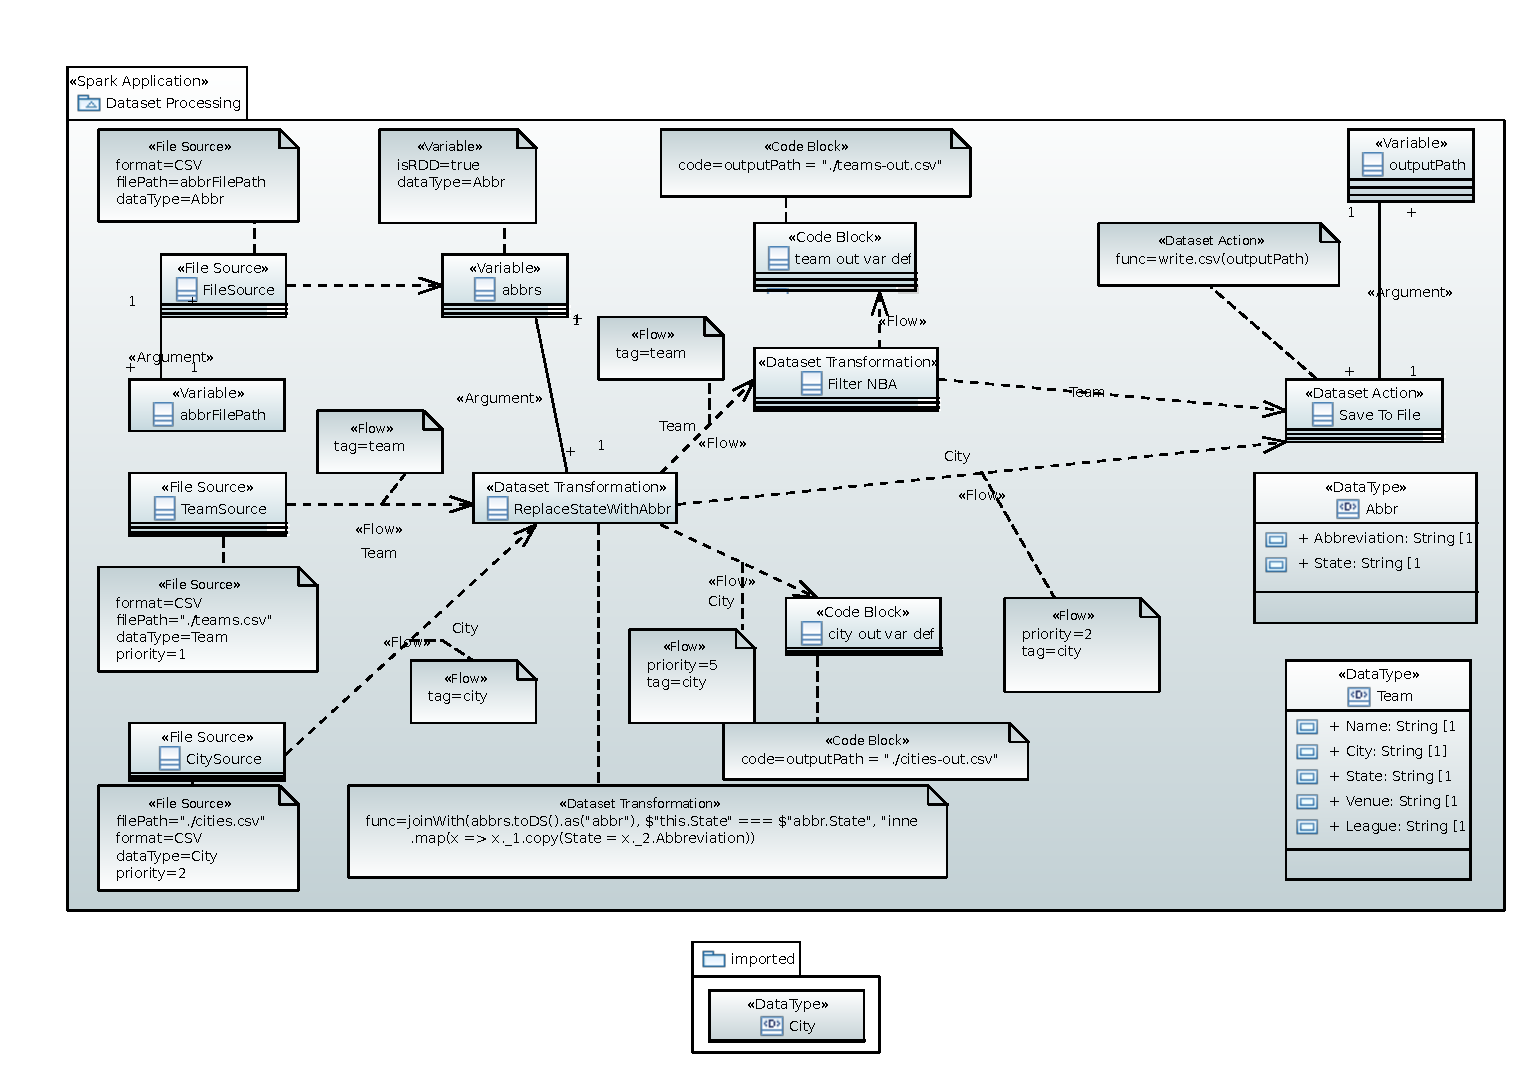
\includegraphics[angle=90,width=1\textwidth]{obrazky-figures/dataset-processing-diagram.pdf}
\label{fig:datsetprocess}
\caption{Dataset processing model diagram}
\centering
\end{figure}


\chapter{Conclusion}

This thesis aimed to design a meta-model for Big Data processing tasks in the Apache Spark framework and develop a tool to generate the target source code of the modeled task. First, I had to get familiar with Spark to accomplish this goal. The essential details to understand the framework are described in chapter \ref{chap:spark}. 

Afterward, the concept I had to get familiar with was Model-Driven Development (MDD). The advantages, disadvantages, and details are discussed in chapter \ref{chap:mdd}. 

After I researched the necessary concepts to understand the problem, I took a look at~already existing tools that try to solve a similar problem. 
An overview of model-driven tools to solve Big Data processing is in chapter \ref{chap:existing}. 

The integral part of this thesis is chapter \ref{chap:design} that goes over the designed meta-model and the reasoning behind specific choices. In addition, it describes the UML Profile diagram and its stereotypes in detail. Furthermore, the choices behind the generated code structure are also discussed. 

The details and highlights of the generator implementation are in chapter \ref{chap:impl}. This chapter brings a further insight into how the implemented Eclipse Acceleo code generator works and how the specific snippets of source code are generated. 

In the last chapter \ref{chap:testing}, a few test cases are presented to make the reader more familiar with the meta-model and to show the specific features in use. The test cases provide a mix between a simple processing pipeline, complex algorithm, and the processing of data with different structures.

Finally, I published the source code, meta-model and model files as open source. The project can be found on GitHub\footnote{\url{https://github.com/MarekSalgovic/spark-m2t-generator}}.
In this next section, I will evaluate the solution and propose a possible future work to~improve the modeling ecosystem.

\section{Evaluation and future work}

I would like to evaluate the designed meta-model, code generator, and the overall approach to Model-Driven Development of Big Data processing tasks. The designed meta-model improved upon the disadvantages of several previous projects. The possibility of modeling a more complex, more readable diagram in a standardized (UML) environment definitely improves the overall MDD approach. The meta-model introduces features that abstract the code behind a relatively comprehensive graphical diagram. 

The first issue with the modeling approach of Spark tasks is that using this meta-model might actually take more time than provisioning the solution with code. In simple processing applications, the generated code does not have enough volume to justify using a~diagram instead of code. Furthermore, code completion and general IntelliSense features of code editors improve productivity more than the diagram's abstraction. The value of~using a diagram comes from introducing a uniform or a standard way to design applications while generating reusable code components. Furthermore, graphical diagrams might also convey more information about the application logic. 

The second issue comes from the robust typing system of the meta-model. While writing Spark code in Scala, the developer can rely on Scala's type inference feature. In addition, code editors would still highlight possible semantic errors. The implemented generator must explicitly generate the type notation to produce reusable, object-oriented code. The fact that the designer must always select appropriate data types in specific model parts also reduces productivity.

Several solutions to these issues come to mind while preserving the diagram's abstract, reusable and straightforward way of expression. As mentioned multiple times in this thesis, a reverse text to model generation tool could heavily improve the productivity of the~workflow. The generated code was designed with this specific idea in mind. Also, OCL constraints could be added to the meta-model to introduce semantic analysis similar to code editors. The data type issue could be solved if the meta-model was designed with a specific target programming language in mind. Spark framework also supports dynamically-typed Python. However, altering the meta-model to exclude the type system would tie it to~a~specific technology. This approach would not work if the meta-model was to be used with a~Java code generator. Java is statically-typed and does not support similar type inference as Scala does.

In conclusion, I consider this project a step in the right direction for a model-driven approach to data processing applications. However, there is still room for several refinements and supporting tools since Model-Driven Development is still a developing methodology.